\documentclass{article}
\usepackage{bm,sectsty,fancyhdr,multicol,lastpage}
\usepackage{amsmath,enumitem,tabularx,textcomp,nccmath,amssymb}
\usepackage{listings} % Insert bullet points
\usepackage[a4paper,left=1cm,right=1cm,top=2cm,bottom=2cm,headsep=0.5cm]{geometry}
\usepackage{xcolor} % Format color in code cells
\usepackage{titlesec} % Format title section
\usepackage{graphicx} % Embed images
\usepackage[document]{ragged2e} % Fix uneven spacing caused in multi col mode

% Define Colors
\definecolor{codegreen}{rgb}{0,0.6,0}
\definecolor{codegray}{rgb}{0.5,0.5,0.5}
\definecolor{codeorange}{rgb}{1,0.49,0}
\definecolor{backcolour}{rgb}{0.95,0.95,0.96}
\lstdefinestyle{mystyle}{
    backgroundcolor=\color{backcolour},
    commentstyle=\color{codegray},
    keywordstyle=\color{codeorange},
    numberstyle=\tiny\color{codegray},
    stringstyle=\color{codegreen},
    %basicstyle=\ttfamily\footnotesize,
    basicstyle=\tiny,
    breakatwhitespace=false,
    breaklines=true,
    captionpos=b,
    keepspaces=true,
    numbers=left,
    numbersep=5pt,
    showspaces=false,
    showstringspaces=false,
    showtabs=false,
    tabsize=2,
    xleftmargin=0pt,
    language=Python,
    label={lst:code},
    mathescape=true,
    gobble=20
}
\lstset{style=mystyle}


% Header and Footer
\pagestyle{fancy}
\fancyhf{}
\fancyhead[L]{ML Cheatsheet}
\fancyfoot[R]{Riten Patel}
\fancyfoot[L]{\LaTeX}
\fancyfoot[C]{\thepage\ of \pageref{LastPage}}
\renewcommand{\headrulewidth}{1.4pt}
\renewcommand{\footrulewidth}{1.4pt}

% Configurations
\sectionfont{\large}
\setlength{\columnsep}{0.5cm}
\setlength{\columnseprule}{1.4pt}
\setlength{\parindent}{0pt}
\setlength{\parskip}{-6pt}
\newcolumntype{Y}{>{\centering\arraybackslash}X}
\setlist[itemize]{nolistsep,left=0pt}
\graphicspath{{./images/}}
\tolerance=9999
\emergencystretch=10pt
\hyphenpenalty=10000
\exhyphenpenalty=100

\begin{document}
\begin{multicols*}{3}
    \raggedcolumns


    % Combinatorics
    \titleformat{\section}
        {\normalfont\fontfamily{phv}\fontsize{10}{0}\bfseries}{\thesection}{1em}{}
        \section{Combinatorics}
    \renewcommand\labelitemi{{\boldmath$\cdot$}}
    \setlist{nolistsep}
    \begin{itemize}[noitemsep]
        \item The study of the number of ways we can arrange a set of elements
        \item Permutations - order matters
        \begin{itemize}
            \item $_{n}P_{r} = \frac{n!}{(n-r)!}$
            \item i.e. count the number of ways runners could split medals
        \end{itemize}
        \item Combinations - order does not matter
        \begin{itemize}
            \item $_{n}C_{r} = {n \choose r} = \frac{n}{r!(n-r)!}$
            \item Symmetrical: $_{n}C_{r} = _{n}C_{n-r}$
        \end{itemize}
    \end{itemize}


    % Bayesian Inference
    \titleformat{\section}
        {\normalfont\fontfamily{phv}\fontsize{10}{0}\bfseries}{\thesection}{1em}{}
        \section{Bayesian Inference}
    \renewcommand\labelitemi{{\boldmath$\cdot$}}
    \setlist{nolistsep}
    \begin{itemize}[noitemsep]
        \item Every set has a set of outcomes and at least two subsets (itself, null)
        \item $A \cup B = A + B - A \cap B $
        \item $P(A|B) = \frac{P(A \cap B)}{P(B)}$
        \item $P(A|B) = \frac{P(B|A)P(A)}{P(B)}$
    \end{itemize}


    % Probability Distribution
    \titleformat{\section}
        {\normalfont\fontfamily{phv}\fontsize{10}{0}\bfseries}{\thesection}{1em}{}
        \section{Probability Distribution}
    \renewcommand\labelitemi{{\boldmath$\cdot$}}
    \setlist{nolistsep}
    \begin{itemize}[noitemsep]
        \item Possible outcomes an event can take and the frequency of occurrence
        \item P(X = x). X = actual outcome of an event and 
        x = one of the possible outcomes.
        \item $\sigma^2 = E((X-\mu)^2) = E(X^2) - \mu^2$
        \item Discrete - finite outcomes
        \begin{itemize}
            \item Uniform - each outcome has an equal chance
            \item Bernoulli - event with two outcomes
            \begin{itemize}
                \item $E(X) = p$
                \item $Var(X) = p(1-p)$
                \item $P(X) = p^x(1-p)^{1-x}$
            \end{itemize}
            \item Binomial - multiple bernoulli trials
            \begin{itemize}
                \item $E(X) = np$
                \item $Var(X) = np(1-p)$
                \item $P(X) = {n \choose x}p^x(1-p)^{n-x}$
            \end{itemize}
            \item Poisson - frequency at which an event occurs
            \begin{itemize}
                \item $E(X) = Var(X) = \lambda$
                \item $P(X) = \frac{\lambda^{x}e^{-\lambda}}{x!}$
            \end{itemize}
        \end{itemize}
        \item Continuous - infinite outcomes 
        \begin{itemize}
            \item Normal: $E(X) = \mu, Var(X) = \sigma^2$
            \item T - small approximation to normal distribution, fat tails 
            \item Chi-squared - for goodness of fit 
            \item Exponential - events rapidly changing early on 
            \begin{itemize}
                \item $E(X) = \frac{1}{\lambda}$
                \item $Var(X) = \frac{1}{\lambda^2}$
                \item $P(X) = \lambda e^{-\lambda x}$
            \end{itemize}
        \end{itemize}
    \end{itemize}


    % Statistics
    \titleformat{\section}
        {\normalfont\fontfamily{phv}\fontsize{10}{0}\bfseries}{\thesection}{1em}{}
        \section{Statistics}
    \renewcommand\labelitemi{{\boldmath$\cdot$}}
    \setlist{nolistsep}
    \begin{itemize}[noitemsep]
        \item Population: collection of all items of interest (N)
        \item Sample - subset of a population (n)
        \item Sample must be random and representative of population
        \item Descriptive
        \begin{itemize}
            \item Two types of data (categorical, numerical)
            \item Two types of measurement \\
            - Qualitative: nominal and ordinal \\
            - Quantitative: interval and ratio \\
            \item Pareto Principle - 80\% of the effect comes from 20\% of the causes
            \item Mean $>$ Median: Skewed right (+)
            \item Mean $<$ Median: Skewed left (-)
            \item Mean = Median: Not Skewed
            \item Mode: peak of distribution
            \item Coefficient of variation: $\frac{\sigma}{\mu}$, useful when 
            comparing 2+ datasets
            \item $Cov(X,Y) = \Sigma_{i=1}^{n}\frac{(x_i-\overline{x})(y_i-\overline{y})}{n-1}$
            \item $Corr(X,Y) = r = \frac{Cov(X,Y)}{\sigma_x\sigma_y}$ \\
            $-1 \leq r \leq 1$
            \item Correlation does not imply causation
        \end{itemize}
        \item Inferential
        \begin{itemize}
            \item Using probability theory to predict population values using sample data
            \item Central Limit Theorem - if you take large random samples from a population, 
            then the distribution of the sample means will be approximately normal regardless 
            of the distribution of the population. \\ 
            Hence, sampling distribution $\sim N(\mu, \frac{\sigma^2}{n})$
            \item Standard Error: standard deviation of sample mean distribution
            \item Good estimators have two properties:
            \begin{itemize}
                \item Efficiency: smallest variance
                \item Bias: expected value = population parameter
            \end{itemize}
            \item Confidence Intervals
            \begin{itemize}
                \item how confident are you population parameter is contained in interval
                surrounding sample estimate
                \item if population variance is unknown, use the t-dist: \\
                $\overline{x} \pm t_{n-1,\alpha/2}\frac{s}{\sqrt{n}}$
                \item if two means, independent samples, and variance is known: \\
                $\sigma_{diff}^2 = \frac{\sigma_e^2}{n_e} + \frac{\sigma_m^2}{n_m}$ \\
                $(\overline{x} - \overline{y}) \pm z_{\alpha/2}\sigma_{diff}$
                \item if two means, independent samples, and variance is unknown: \\
                $s_p^2 = \frac{(n_x-1)s_x^2 + (n_y - 1)s_y^2}{n_x n_y -2}$ \\
                $(\overline{x}-\overline{y}) \pm t_{n_x+n_y-2,\alpha/2}\sqrt{\frac{s_p^2}{n_x} + \frac{s_p^2}{n_y}}$
            \end{itemize}
            \item Hypothesis Testing 
            \begin{itemize}
                \item Hypothesis: idea that can be tested
                \item Research is trying to reject the null Hypothesis
                \item Type I error: rejecting a true null hypothesis ($\alpha$)
                \item Type II error: accepting a false null hypothesis ($\beta$)
                \item p-value: smallest level of significance we can still reject 
                the null hypothesis given the observed sample statistic.
            \end{itemize}
        \end{itemize}
    \end{itemize}


    % K Nearest Neighbors
    \titleformat{\section}
        {\normalfont\fontfamily{phv}\fontsize{10}{0}\bfseries}{\thesection}{1em}{}
        \section{K-Nearest Neighbors}
    \renewcommand\labelitemi{{\boldmath$\cdot$}}
    \setlist{nolistsep}
    \begin{itemize}[noitemsep]
        \item For every test observation find its k closest training 
        observations. Then, take a majority vote or average on their class labels 
        and assign its label to the test observation.
        \item $P(Y=j) = \frac{1}{K}\Sigma_{i \in N_0}I(y_i=j)$
    \end{itemize}

    % Simple Linear Regression
    \titleformat{\section}
        {\normalfont\fontfamily{phv}\fontsize{10}{0}\bfseries}{\thesection}{1em}{}
        \section{Simple Linear Regression}
    \renewcommand\labelitemi{{\boldmath$\cdot$}}
    \setlist{nolistsep}
    \begin{itemize}[noitemsep]
        \item A linear approximation of a causal relationship between two variables
        \item $y = \beta_0 + \beta_1 x_1 + \epsilon$
        \item Correlation is the degree of relationship between two variables whereas
        regression is how one variable affects another
        \item Correlation is symmetric. Regression is one-way 
        \item Correlation is visualized as a single point on a scatter plot. 
        Regression is a best fit line on a scatter plot.
        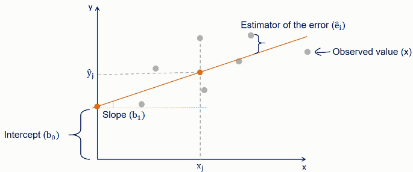
\includegraphics[width=\linewidth]{simple_linear_regression_chart}
        \item $SST = \Sigma_{i=1}^n(y_i-\overline{y})^2$: 
        total variability of dataset
        \item $SSR = \Sigma_{i=1}^n(\hat{y_i}-\overline{y})^2$: 
        variability explained by regression
        \item $SSE = \Sigma_{i=1}^n(\hat{y_i} - y_i)^2$:
        unexplained variability
        \item $SST = SSR + SSE$
        \item Ordinary Least Squares (OLS) to estimate parameters such that SSE 
        is minimized.
        \item $R^2 = \frac{SSR}{SST}$: Proportion of total variability explained by 
        regression
        \item What's a good $R^2$?:
        \begin{itemize}
            \item goodness of fit: [0.2,0.9]
            \item physics/chemistry: [0.7, 0.9]
            \item social sciences: [0.2]
            \item generally depends on the topic and number of independent variables
        \end{itemize}
    \end{itemize}


    % Multiple Linear Regression
    \titleformat{\section}
        {\normalfont\fontfamily{phv}\fontsize{10}{0}\bfseries}{\thesection}{1em}{}
        \section{Multiple Linear Regression}
    \renewcommand\labelitemi{{\boldmath$\cdot$}}
    \setlist{nolistsep}
    \begin{itemize}[noitemsep]
        \item $y = \beta_0 + \beta_1x_1 + \beta_2x_2 + ... + \epsilon$
        \item more variables, more explanatory power
        \item $R_{adj}^2 = 1 - \frac{SSE/(n-K)}{SST/(n-1)}$
        \item F-Test for overall significance: \\
        $H_0: \beta_1 = \beta_2 = ... = \beta_k = 0$ \\
        $H_1$: at least one $\beta_i \neq 0$
        \item OLS Assumption
        \begin{itemize}
            \item Linearity: relationship between the dependent variable y and 
            independent variable x is linear.
            \item Normality: All variables must be multivariate normal otherwise
            you need a non-linear transformation.
            \item No multicollinearity: All variables are independent of each other
            \item No autorrelation: Observations must be independent of each other
            \item Homoscedasticity: Variance of the error terms given x is constant
        \end{itemize}
        \item number of dummy variables = number of categories - 1. Each dummy 
        has a value of 0 or 1.
        \item Feature Scaling (Standardization)
        \begin{itemize}
            \item to ensure no one variable is more important than the other
            \item Ex. Euro Exchange rate vs. daily trading volumes
        \end{itemize}
        \item Underfitting and Overfitting
        \begin{itemize}
            \item Overfitting - training accuracy is high but testing accuracy is low. 
            Model is too foucsed on the training set that it has "missed the point". 
            You modeled the noise.
            \item Underfitting - Model has not captured the undelrying logic of the 
            data. To overcome, split the data into training, testing, and shuffle 
            the data.
            \item Bias - Variance Tradeoff: A balance between an underfitted and 
            an overfitted model broken by model complexity.
        \end{itemize}
    \end{itemize}


    % Logistic Regression
    \titleformat{\section}
        {\normalfont\fontfamily{phv}\fontsize{10}{0}\bfseries}{\thesection}{1em}{}
        \section{Logistic Regression}
    \renewcommand\labelitemi{{\boldmath$\cdot$}}
    \setlist{nolistsep}
    \begin{itemize}[noitemsep] 
        \item Regressing probability of a categorical variable
        \item Assumptions same as SLR except linearity is violated
        \item Can't use linear regression because output would be outside [0,1]
        \item So use sigmoid: $\mathbb{R} \rightarrow [0,1]$
        \item PDF Derivation
        \begin{itemize}
            \item Take sigmoid: $\delta(t) = \frac{1}{1+e^{-t}}$
            \item Take SLR: $t = \beta_0 + \beta_1x$
            \item Plug in: $\delta(x) = \frac{1}{1+e^{-(\beta_0+\beta_1x)}}$
            \item Logit: $log(\frac{p(x)}{1-p(x)}) = \beta_0 + \beta_1x$
        \end{itemize}
        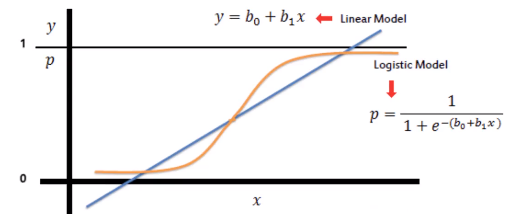
\includegraphics[width=\linewidth]{q26_logistic_regression}
        \item Use MLE for parameter estimation
        \begin{itemize}
            \item Estimates how likely model describes real underlying 
            relationship of variables
            \item Bigger the likelihood, higher the probability the model 
            is correct
            \item Easier to maximize log likelihood
        \end{itemize}
        \item Log likelihood ratio test: for overall model significance
        \item Confusion matrix: how confused model is 
    \end{itemize}


    % Support Vector Machines
    \titleformat{\section}
        {\normalfont\fontfamily{phv}\fontsize{10}{0}\bfseries}{\thesection}{1em}{}
        \section{Support Vector Machines}
    \renewcommand\labelitemi{{\boldmath$\cdot$}}
    \setlist{nolistsep}
    \begin{itemize}[noitemsep]
        \item SVM attempts to find a hyperplane that separates classes 
        by maximizing the margin
        \item See diagram. The filled in points are the support vectors of the 
        decision hyperplane.
        \item So, really low x1 and x2 would be classified as a square and 
        realy high x1 and x2 would be classified as a circle.
        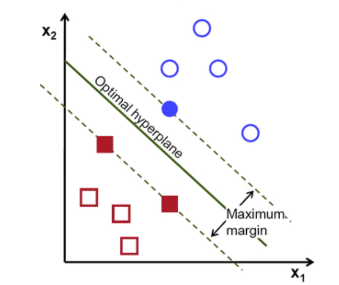
\includegraphics[width=\linewidth]{q31_svm_linear}
        \item If we have a non-linear decision boundary, we'll 
        use the kernel trick: map linear non-separable inputs into 
        a higher dimension where they become more easily seperable.
        \item $\Phi: \mathbb{R}^2 \rightarrow \mathbb{R}^3$ \\
        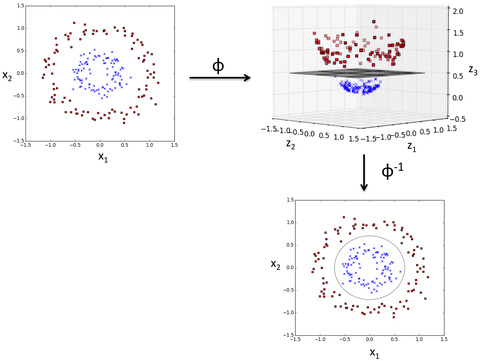
\includegraphics[width=\linewidth]{q31_svm_nonlinear}
    \end{itemize}


    % Decision Trees
    \titleformat{\section}
        {\normalfont\fontfamily{phv}\fontsize{10}{0}\bfseries}{\thesection}{1em}{}
        \section{Decision Trees}
    \renewcommand\labelitemi{{\boldmath$\cdot$}}
    \setlist{nolistsep}
    \begin{itemize}[noitemsep]
        \item Partition the feature space into regions and computing the 
        mean/mode of the training responses (regression) in that region 
        in classifying the test observation. \\
        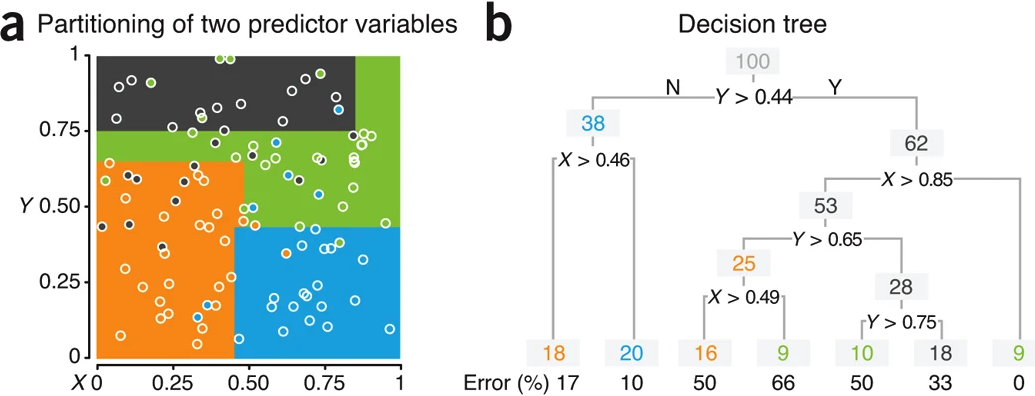
\includegraphics[width=\linewidth]{cart_chart}
        \item Algorithm \\
        - High Level: Split target class into the purest possible 
        children nodes. Measure of purity is called the information. \\
        - Node purity: node contains predominantly observations 
        from a single class
        \begin{enumerate}
            \item Use recursive binary splitting to grow a large tree. 
            Stop when each terminal node has fewer than some minimum 
            number of observations.
            \item Node impurity splitting metrics:
                \begin{itemize}
                    \item Let $\hat{p}_{mk}$ be the proportion of 
                    training observations from the $m^{th}$ region 
                    from the $k^{th}$ class. We want small values 
                    for gini index, cross entropy, error.
                    \item Categorical Target \\
                    - Information Gain: Entropy before - Entropy after \\
                    $Entropy= -\Sigma_{k=1}^K\hat{p}_{mk}log\hat{p}_{mk}$ \\
                    - Gini Index: \\
                    $G = \Sigma_{k=1}^K\hat{p}_{mk}(1-\hat{p}_{mk})$ \\
                    - Classification Error: \\
                    $E = 1 - max(\hat{p}_{mk})$ \\
                    \item Continuous Target \\
                    - Variance Reduction: \\
                    $S(T) - S(T,X) = $ \\
                    $\frac{1}{n}\Sigma_{i=1}^n(y_i - \overline{y})^2 - \Sigma_{c \in X}P(c)S(c)$
                \end{itemize}
            \item Prune the tree or use Random Forest to prevent overfitting
        \end{enumerate}
    \end{itemize}


    % Random Forest
    \titleformat{\section}
        {\normalfont\fontfamily{phv}\fontsize{10}{0}\bfseries}{\thesection}{1em}{}
        \section{Random Forest}
    \renewcommand\labelitemi{{\boldmath$\cdot$}}
    \setlist{nolistsep}
    \begin{itemize}[noitemsep]
        \item To increase the predictive power of decision trees.
        \item Algorithm 
        \begin{enumerate}
            \item Construct B regresion trees using B bootstrapped training 
            sets (sampling with replacement), and average the resulting 
            predictions or take a majority vote for classificaiton problems
            \item Let trees be deep and unpruned
            \item For each tree, use 2/3 as training, 1/3 as OOB observations
            \item Predict response on the OOB observations. Repeat on all B trees
            \item Average predicted responses or take majority vote to get 
            a single OOB prediction for each observation
            \item Compute the overall OOB MSE or classification error
        \end{enumerate}
        \item Random Forest de-correlates trees:
        \begin{itemize}
            \item Each time a split is considered, a random sample of m 
            predictors is chosen as split candidates from the full set of 
            p predictors ($m \approx \sqrt{p}$)
            \item Trees will not look similar to each other since 
            strong predictors, which otherwise would be present in most trees, 
            will be removed
        \end{itemize}
        \item Can find important variables
        \begin{itemize}
            \item Record the amount the RSS/Gini index has decreased
            due to splits over a predictor, averaged across all B trees.
            \item Large values indicate important variables
        \end{itemize}
    \end{itemize}


    % Cluster Analysis
    \titleformat{\section}
        {\normalfont\fontfamily{phv}\fontsize{10}{0}\bfseries}{\thesection}{1em}{}
        \section{Cluster Analysis}
    \renewcommand\labelitemi{{\boldmath$\cdot$}}
    \setlist{nolistsep}
    \begin{itemize}[noitemsep]
        \item Dividing observations into groups based on features
        \item Goal is to maximize similarity of observations within a cluster 
        and maximize dissimilarity between clusters
        \item Curse of dimensionality: an observation has no nearby 
        neighbors (i.e. p $>$ n). This will drastically increase the error 
        rate and computation time. Use Manhattan distance if this occurs.
        \item Distance Metrics:
        \begin{itemize}
            \item Euclidean \\
            - Find shortest path between points \\
            - $\sqrt{\Sigma_{i=1}^k(x_i-y_i)^2}$ \\
            \item Manhattan \\
            - Find shortest zig-zag path between points \\
            - $\Sigma_{i=1}^k|x_i - y_i|$ \\
            \item Hamming \\
            - Find distance between two binary data strings \\
            - Used for categorical variables \\
            - $D_H = \Sigma_{i=1}^k|x_i - y_i|$ \\
        \end{itemize}
        \item Examples:
        \begin{itemize}
            \item Market segmentation
            \item Data Exploration
            \item Image segmentation
            \item Object recognition
        \end{itemize}
    \end{itemize}


    % K-Means Clustering
    \titleformat{\section}
        {\normalfont\fontfamily{phv}\fontsize{10}{0}\bfseries}{\thesection}{1em}{}
        \section{K-Means Clustering}
    \renewcommand\labelitemi{{\boldmath$\cdot$}}
    \setlist{nolistsep}
    \begin{itemize}[noitemsep]
        \item Algorithm
        \begin{enumerate}
            \item Choose number of clusters \\
            - WCSS: make as small as possible \\
            - Elbow method: plot of WCSS vs. num clusters. 
            Look for diminishing improvements
            \item Specify the cluster seeds
            \item Assign each point to a centroid based on distance
            \item Adjust centroids
            \item Repeat steps 4 and 5 until a stopping criterion is met.
            It can be (1) centroids don't change much, (2) points remain 
            in same cluster, (3) max number of iterations is reached
        \end{enumerate}
        \item Pros 
        \begin{itemize}
            \item Simple to understand
            \item Fast to cluster
            \item Easy to implement
            \item Always yields a result
        \end{itemize}
        \item Cons
        \begin{itemize}
            \item Need to pick a K
            \item Sensitive to initialization $\rightarrow$ k-means++
            \item Sensitive to outliers $\rightarrow$ remove them
            \item Produces spherical vs. elliptic solutions
            \item Must standardize to put variables on equal footing
        \end{itemize}
    \end{itemize}


    % Hierarchical Clustering
    \titleformat{\section}
        {\normalfont\fontfamily{phv}\fontsize{10}{0}\bfseries}{\thesection}{1em}{}
        \section{Hierarchical Clustering}
    \renewcommand\labelitemi{{\boldmath$\cdot$}}
    \setlist{nolistsep}
    \begin{itemize}[noitemsep]
        \item Two forms of Clustering
        \begin{enumerate}
            \item Agglomerative (bottom-up) \\
            - Easy to solve \\
            - Start at bottom and pair closest observations into a cluster.
            Use euclidean distance to iteratively group clusters until there's
            only one. \\
            \item Divisive (top-down) \\
            - Have to consider all possibilities until there's one cluster \\
        \end{enumerate}
        \item Dendrogram
        \begin{itemize}
            \item Tree representation. Start from bottom and work your way 
            to the top. It tells you how similar clusters are to each 
            other based on the distance between the links.
            \item Draw the line when the distance between the clusters is 
            too big \\
            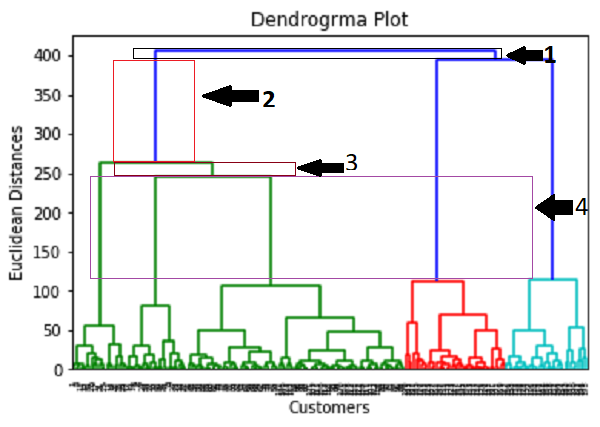
\includegraphics[width=\linewidth]{hiearchical_clustering_dendrogram} \\
        \end{itemize}
        \item Pros
        \begin{itemize}
            \item Shows linkages between clusters
            \item Understand the data much, much better
            \item No need to preset the number of clusters (k-means)
        \end{itemize}
        \item Cons 
        \begin{itemize}
            \item Huge dendrogram
            \item Computationally intensive
        \end{itemize}
    \end{itemize}


    % DBSCAN
    \titleformat{\section}
        {\normalfont\fontfamily{phv}\fontsize{10}{0}\bfseries}{\thesection}{1em}{}
        \section{DBSCAN}
    \renewcommand\labelitemi{{\boldmath$\cdot$}}
    \setlist{nolistsep}
    \begin{itemize}[noitemsep]
        \item Density-based spatial clustering of applications with noise
        \item Clusters are continuous regions of high density; low 
        density regions separate clusters. \\
        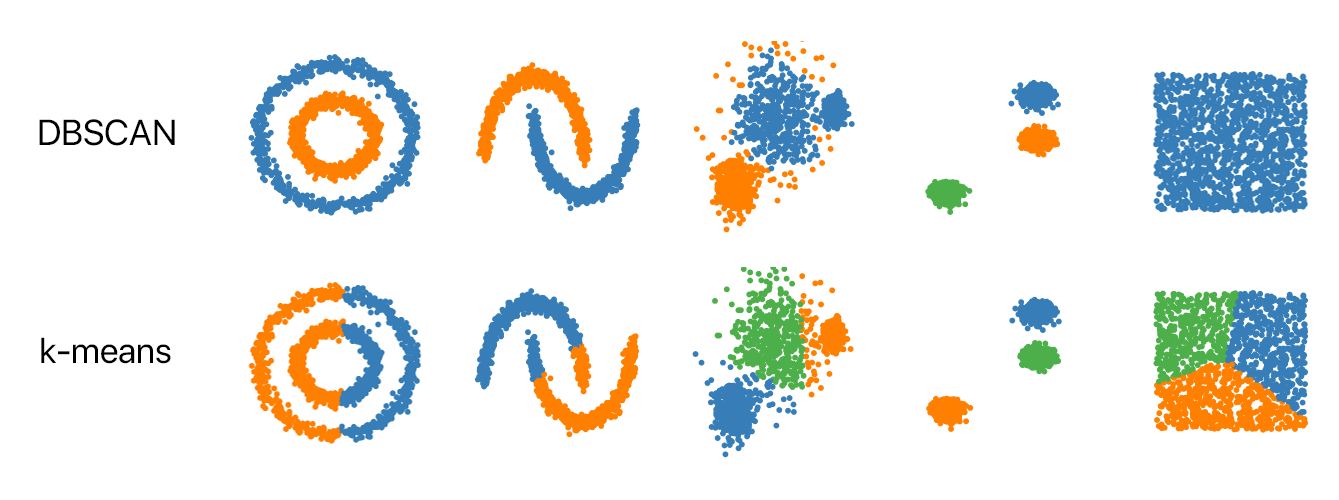
\includegraphics[width=\linewidth]{dbscan}
        \item Two hyperaparameters to specify
        \begin{itemize}
            \item Epsilon: distance metric to locate 
            points/check density in neighborhood of any point \\
            Optimal: plot distance of every observation and neighbors.
            Select epsilon at point of maxmimum curvature.
            \item minPoints: minimum number of points clustered together 
            for a region to be considered dense
        \end{itemize}
        \item Pros 
        \begin{itemize}
            \item Outliers easily identifiable
            \item Can take irregular shapes 
            \item Don't need to preset number of clusters
        \end{itemize}
        \item Cons
        \begin{itemize}
            \item Bad for sparse datasets
            \item Sensitive to hyperaparameters
            \item Can't partition for multiprocessing
        \end{itemize}
    \end{itemize}


    % Linear Algebra
    \titleformat{\section}
        {\normalfont\fontfamily{phv}\fontsize{10}{0}\bfseries}{\thesection}{1em}{}
        \section{Linear Algebra}
    \renewcommand\labelitemi{{\boldmath$\cdot$}}
    \setlist{nolistsep}
    \begin{itemize}[noitemsep]
        \item Everything is a tensor
        \item Tensors have ranks (number of axes)
        \item Scalar: 1x1. Rank=0
        \item Vector: mx1. Rank=1
        \item Matrix: m*n. Rank=2
        \item Triad: m*n*k. Rank=3
        \item Why is linear algebra useful?
        \begin{itemize}
            \item Vectorization for computational efficiency
            \begin{itemize}
                \item Can by-pass using a for-loop and take 
                advantage of the SIMD paradigm.
                \item SIMD: Single Instruction - Multiple Data, 
                a method for combining multiple operations into a 
                single computer instruction
                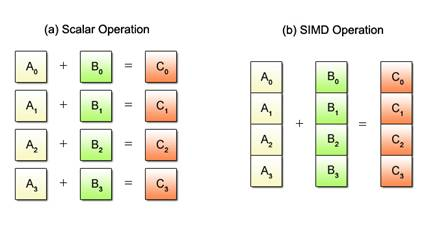
\includegraphics[width=\linewidth]{simd_graphic}
            \end{itemize}
            \item Dimensionality reduction
            \begin{itemize}
                \item "curse of dimensionality": when p $>$ n. The sample 
                is too small and too many inputs can dramatically impact
                model performance.
                \item As a solution, use matrix factorization (LU, QR, Eigendecomposition, 
                SVD) and PCA
            \end{itemize}
            \item Computer vision
            \begin{itemize}
                \item All images are stored as a matrix with values between 
                0 and 255. Colored ones stored on the RGB system have 
                three layers, stored as a tensor of rank 3: m*n*3.
            \end{itemize}
        \end{itemize}
    \end{itemize}


    % Deep Learning
    \titleformat{\section}
        {\normalfont\fontfamily{phv}\fontsize{10}{0}\bfseries}{\thesection}{1em}{}
        \section{Deep Learning}
    \renewcommand\labelitemi{{\boldmath$\cdot$}}
    \setlist{nolistsep}
    \begin{itemize}[noitemsep]
        \item Types of Machine Learning
        \begin{itemize}
            \item Supervised
            \item Unsupervised
            \item Reinforcement
        \end{itemize}
        \item Linear Model
        \begin{itemize}
            \item $Y = XW + B$
            \item Multiple inputs, outputs, observations \\
            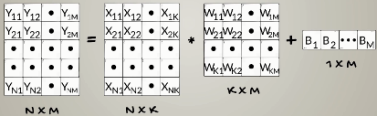
\includegraphics[width=\linewidth]{linear_model_matrix} \\
            \item Deep Neural Networks are helpful for finding nonlinearly 
            separable boundaries to data
        \end{itemize}
    \end{itemize}


    % TensorFlow
    \titleformat{\section}
        {\normalfont\fontfamily{phv}\fontsize{10}{0}\bfseries}{\thesection}{1em}{}
        \section{TensorFlow}
    \renewcommand\labelitemi{{\boldmath$\cdot$}}
    \setlist{nolistsep}
    \begin{itemize}[noitemsep]
        \item Software developed by Google that utilizes GPU in 
        addition to CPU for deep learning models. Optionally, 
        it can use TPUs for models.
        \item Why use GPUs over CPUs?
        \begin{itemize}
            \item Are optimized for parallel computing
            \item Have thousands of cores 
            \item Has multiple hyperthreads per core
        \end{itemize}
        \item Why use CPUs over GPUS?
        \begin{itemize}
            \item CPUs process data sequentially
            \item They do not know what instruction will be next (i.e. 
            input from keyboard, mouse, ...)
            \item Has resources to manage an Operating System
        \end{itemize}
    \end{itemize}


    % Neural Networks
    \titleformat{\section}
        {\normalfont\fontfamily{phv}\fontsize{10}{0}\bfseries}{\thesection}{1em}{}
        \section{Neural Networks}
    \renewcommand\labelitemi{{\boldmath$\cdot$}}
    \setlist{nolistsep}
    \begin{itemize}[noitemsep]
        \item Neural Network: set of algorithms (supervised, unsupservised, reinforcement) 
        trying to recognize patterns and relationships within data \\
        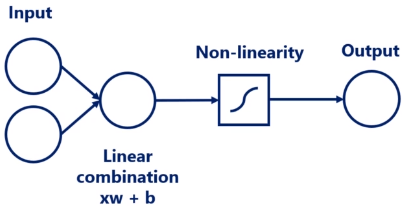
\includegraphics[width=\linewidth]{neural_network_architecture} \\
        \item Deep Neural Network: A neural nework with one or more hidden layers \\
        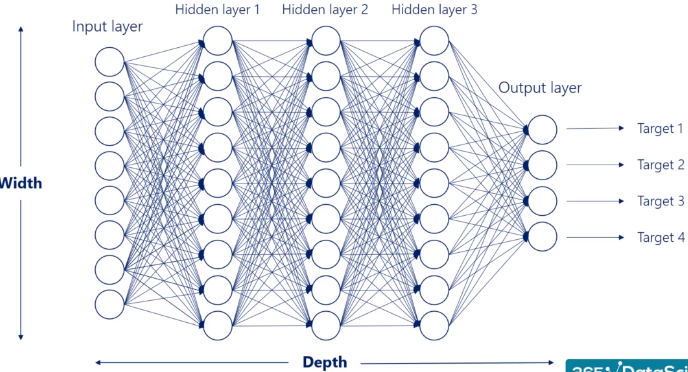
\includegraphics[width=\linewidth]{deep_neural_network2} \\
        \item Hyperparameters: pre-set by the practitioner
        \item Parameters: set by optimization
        \item Why do we need non-linearites?
        \begin{itemize}
            \item Two consecutive linear transformations are equal to a single one,
            meaning hidden layers are useless
            \item Use non-linearities to find complex relationships
        \end{itemize}
        \item Four common activation functions. 
        All are monotonic, continuous, and differentiable
        \begin{itemize}
            \item Sigmoid: $(-\infty,+\infty) \rightarrow (0,1)$ \\
            $f(x) = \frac{1}{1+e^{-x}}$ \\
            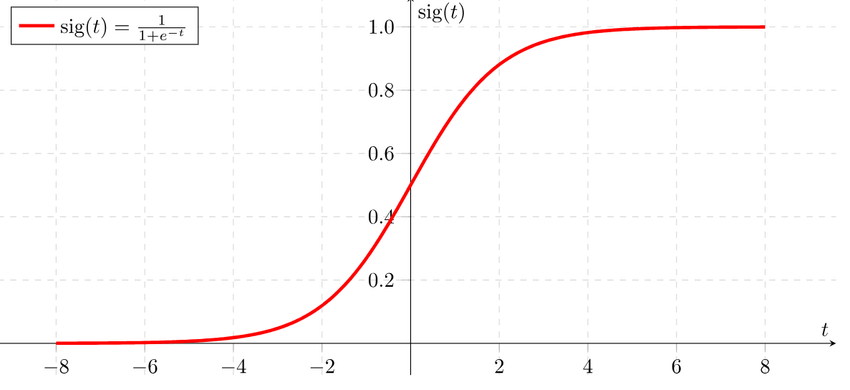
\includegraphics[width=\linewidth]{sigmoid_function} \\
            \item Tanh: $(-\infty,+\infty) \rightarrow (-1,1)$ \\
            $f(x) = \frac{e^x-e^{-x}}{e^x+e^{-x}}$ \\
            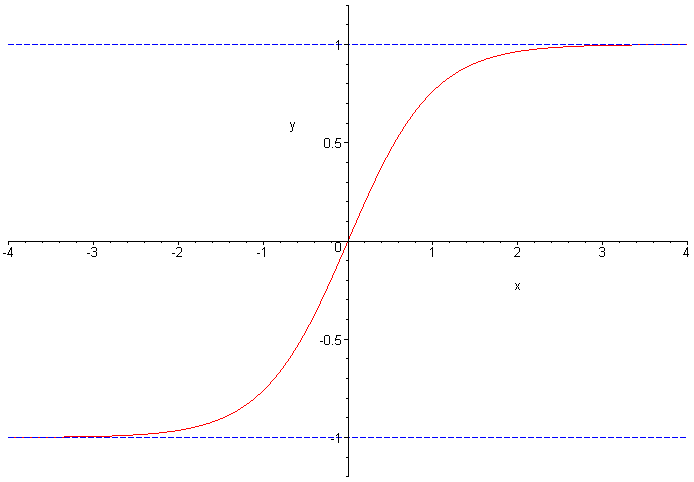
\includegraphics[width=\linewidth]{tanh_function} \\
            \item ReLu: $(-\infty,+\infty) \rightarrow (0,+\infty)$ \\
            $f(x) = max(0,x)$ \\
            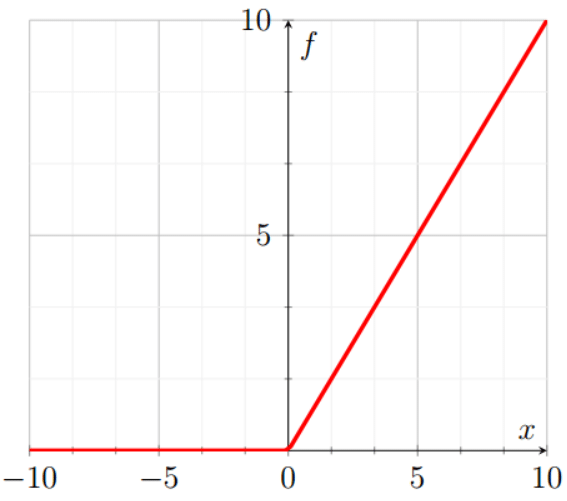
\includegraphics[width=\linewidth]{relu_function} \\
            \item Softmax: $(-\infty,+\infty) \rightarrow (0,1)$ \\
            $f(x) = \frac{e^{z_i}}{\Sigma_{j=1}^Ke^{z_j}}$ \\
            Softmax is most often used in the final output layer. 
            The output layer has values between 0 and 1. The function transforms 
            a bunch of numbers into a valid probability distribution. \\
        \end{itemize}
        \item Backpropagation
        \begin{itemize}
            \item Technique to update the weights and biases in a neural 
            network in a way to minimize the loss function
            \item Vanishing Gradient: gradient diminishes as it 
            propagates backwkard through the network. By the 
            time it reaches layers close to the input, it may have 
            little effect. Use ReLu as a solution because the 
            derivative will not be anything near 0.
            \item Exploding gradient: gradient exponentially increases as it's
            backpropagated through the network. Solution (1) gradient clipping 
            if their norm exceeds a threshold, (2) redesign the network 
            and use smaller batch sizes and LSTMs
        \end{itemize}
        \item Loss function - how well model's outputs
        match the true outputs
        \begin{itemize}
            \item Regression: L2 RSS Norm \\
            - $L = \Sigma_{i=1}^N(y_i-\hat{y}_i)^2$
            \item Classification - Cross Entropy \\
            - $L = -\Sigma_{i=1}^N\Sigma_{j=1}^My_{i,j}ln(p_{i,j})$
        \end{itemize}
        \item Gradient Descent: algorithm to find the minimum of  
        a loss function. Takes small steps in direction of steepest descent.
        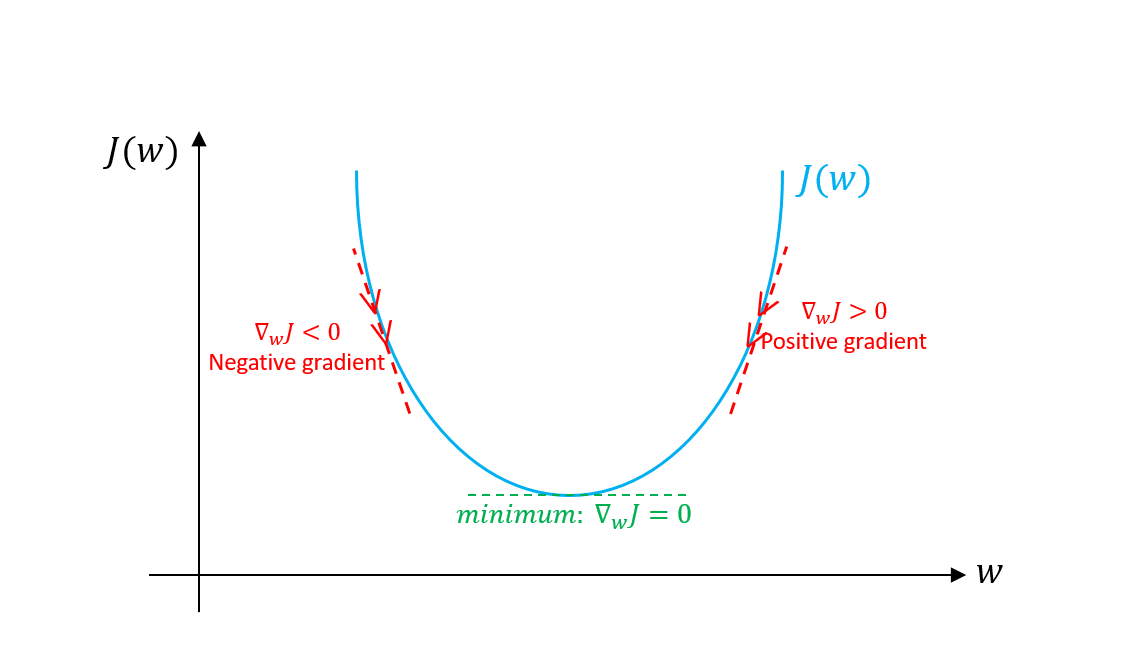
\includegraphics[width=\linewidth]{gradient_descent}
        \begin{itemize}
            \item $x_{i+1} = x_i - \gamma f^`(x_i)$
            \item $\gamma$ is the learning rate (speed of minimization)
            \item If learning rate is too low, it wil take forever to 
            converge. If too high, we'll oscillate around the minimum 
            but not converge.
        \end{itemize}
        \item Batch size: number of samples needed to update parameters
        \begin{itemize}
            \item (BGD) Batch gradient descent: use
            total number of training examples
            \item (SGD) Stochastic gradient descent: batch size = 1 training example 
            \item (MGD) Mini-batch gradient descent: batch size = 
            subset of total number of training examples. 
            \item MGD $>$ SGD $>$ BGD. BGD may not fit into memory and get 
            stuck at a local minima, SGD with fewer data points jerks model 
            out of local minima but is very noisy, MGD is a balance between
            the two.
        \end{itemize}
        \item Epoch: one full pass through training dataset
    \end{itemize}


    % Model Evaluation and Selection
    \titleformat{\section}
        {\normalfont\fontfamily{phv}\fontsize{10}{0}\bfseries}{\thesection}{1em}{}
        \section{Model Evaluation and Selection}
    \renewcommand\labelitemi{{\boldmath$\cdot$}}
    \setlist{nolistsep}
    \begin{itemize}[noitemsep]
        \item Bias-Variance Tradeoff
        \begin{itemize}
            \item $y = f(x) + \epsilon$
            \item $\epsilon$ = Bias + Variance + Irreducible error
            \item Bias: How often model's predicted values come to 
            the true underlying f(x) values
            \item Variance: how often does prediction error change as 
            you change the training dataset
            \item Irreducible error: due to inherently noisy observation process
        \end{itemize}
        \item Model Complexity and Overfitting
        \begin{itemize}
            \item Overfitting remedies: \\
            - Regularization (Shrinkage): Add a penalty to the objective function.
            The penalty shrinks coefficients. \\
            - L1 (Lasso): $\Sigma_{i=1}^N (y_i - \hat{y}_i)^2 + \gamma\Sigma_{j=1}^p|\beta_j|$ \\
            - L2 (Ridge): $\Sigma_{i=1}^N (y_i - \hat{y}_i)^2 + \gamma\Sigma_{j=1}^p\beta_j^2$ \\
            - L1 can zero-out parameters, L2 can shrink but not zero-out
        \end{itemize}
        \item Interpretability
        \begin{itemize}
            \item In the real world, explaining the model is important 
            and choosing a simpler model in fields like healthcare, 
            IRS, ... is important.
        \end{itemize}
    \end{itemize}


\end{multicols*}
\end{document}